\documentclass{article}
\usepackage[utf8]{inputenc}

\usepackage[margin=1.3in]{geometry}
 
 
\usepackage{hyperref}
\hypersetup{
    colorlinks=true,
    linkcolor=blue,
    filecolor=blue,      
    urlcolor=blue,
}
\urlstyle{same}
  
\usepackage{schemabloc}
\usetikzlibrary{circuits}

\usepackage[bottom]{footmisc}
\usepackage{pgf}
\usepackage{tikz}
\usetikzlibrary{arrows,automata}
\usepackage{verbatim}
 
% \title{Machine~Learning~Engineer~Nanodegree Capstone Proposal: Machine Learning for Functional 
\title{Capstone Proposal: Machine~Learning~for~Functional~Verification}
\author{Alberto Guasco}
% \date{\today}
 
\begin{document}
 
\maketitle

The project I will develop for concluding the Nanodegree concerns the usage of machine learning techniques for improving functional verification. My goal is to understand if a highly dimensional system such as a generic piece of hardware can be verified more efficiently using intelligent stimulus generation.
 
\paragraph*{Background}

% Student briefly details background information of the domain from which the project is proposed. Historical information relevant to the project should be included. It should be clear how or why a problem in the domain can or should be solved. Related academic research should be appropriately cited. A discussion of the student's personal motivation for investigating a particular problem in the domain is encouraged but not required.

In the \href{http://www.asic-world.com/verilog/design_flow1.html}{RTL design flow}, \href{https://en.wikipedia.org/wiki/Functional_verification}{functional verification} is a key step  because it requires considerable efforts and ensures the manufacturer to have a product that respects all the specifications and functionalities designed. The verification is considered completed if we can estimate that on the device under testing (hereafter DUT) all checkers have not failed and the DUT has been fully stimulated. Some years ago it was feasible to detail all possible DUT's states and then check one-by-one if they have been reached almost once, or precompute which series of stimuli are needed for reaching a certain state. Right now for more complex DUT (such as modern microprocessors) these scenarios are far from reality. The complexity of DUT is increasing (following \href{https://en.wikipedia.org/wiki/Moore%27s_law}{Moore's Law}), it's really difficult to list all possible states and find an efficient way to stimulate them in order to complete the verification in the shortest possible time.
Differently from the problems seen during the Nanodegree, this one doesn't describe any daily issue. Anyway it really motivates me as I worked on this domain: I experienced this problem and I'm sure that machine learning will become a standard for solving it. Moreover it will be interesting to see if the results of this work can be applied on other kind of problems.

\paragraph{Problem Statement}
% Student clearly describes the problem that is to be solved. The problem is well defined and has at least one relevant potential solution. Additionally, the problem is quantifiable, measurable, and replicable.
Given a known DUT and given the list of states that the DUT has to reach, we propose to use machine learning for stimulate the DUT in order to reach all states in the shortest possible time.
The DUT is an ensemble of sequential and combinatorial logic: we force some binary values in the inputs, the internal registers change their states and the outputs are the results of operations done on the registers values.
\tikzset{every picture/.style={line width=0.75pt}} %set default line width to 0.75pt        
\begin{figure}
\begin{center}
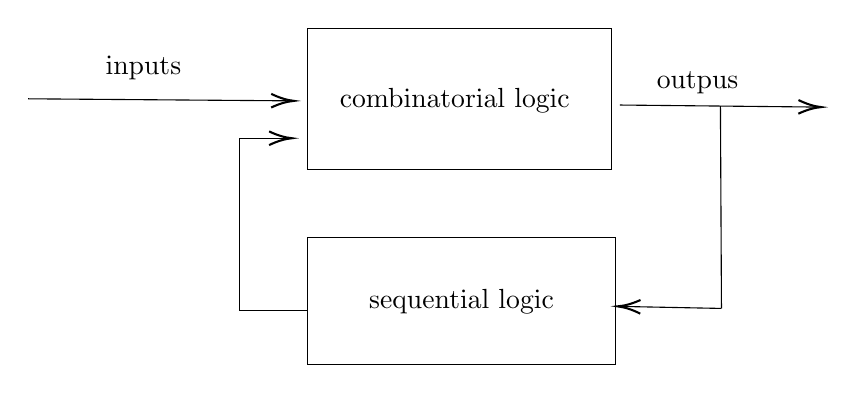
\begin{tikzpicture}[x=0.75pt,y=0.75pt,yscale=-1,xscale=1]
%uncomment if require: \path (0,300); %set diagram left start at 0, and has height of 300

%Straight Lines [id:da9594583335701603] 
\draw    (101.5,129) -- (227.5,129.98) ;
\draw [shift={(229.5,130)}, rotate = 180.45] [color={rgb, 255:red, 0; green, 0; blue, 0 }  ][line width=0.75]    (10.93,-3.29) .. controls (6.95,-1.4) and (3.31,-0.3) .. (0,0) .. controls (3.31,0.3) and (6.95,1.4) .. (10.93,3.29)   ;

%Shape: Rectangle [id:dp94563734044778] 
\draw   (236,95) -- (382.5,95) -- (382.5,163) -- (236,163) -- cycle ;
%Straight Lines [id:da5845685599472759] 
\draw    (386.5,132) -- (481.5,132.98) ;
\draw [shift={(483.5,133)}, rotate = 180.59] [color={rgb, 255:red, 0; green, 0; blue, 0 }  ][line width=0.75]    (10.93,-3.29) .. controls (6.95,-1.4) and (3.31,-0.3) .. (0,0) .. controls (3.31,0.3) and (6.95,1.4) .. (10.93,3.29)   ;

%Shape: Rectangle [id:dp11834384088600869] 
\draw   (236,196) -- (384.5,196) -- (384.5,257) -- (236,257) -- cycle ;
%Straight Lines [id:da3011906563331679] 
\draw    (435,132.5) -- (435.5,230) ;


%Straight Lines [id:da2080054398331841] 
\draw    (435.5,230) -- (387.5,229.04) ;
\draw [shift={(385.5,229)}, rotate = 361.15] [color={rgb, 255:red, 0; green, 0; blue, 0 }  ][line width=0.75]    (10.93,-3.29) .. controls (6.95,-1.4) and (3.31,-0.3) .. (0,0) .. controls (3.31,0.3) and (6.95,1.4) .. (10.93,3.29)   ;

%Straight Lines [id:da2418080495725663] 
\draw    (203.5,231) -- (236.5,231) ;


%Straight Lines [id:da2403153951084427] 
\draw    (203.5,148) -- (203.5,231) ;


%Straight Lines [id:da26911747717628987] 
\draw    (203.5,148) -- (226.5,148) ;
\draw [shift={(228.5,148)}, rotate = 180] [color={rgb, 255:red, 0; green, 0; blue, 0 }  ][line width=0.75]    (10.93,-3.29) .. controls (6.95,-1.4) and (3.31,-0.3) .. (0,0) .. controls (3.31,0.3) and (6.95,1.4) .. (10.93,3.29)   ;


% Text Node
\draw (157,114) node  [align=left] {inputs};
% Text Node
\draw (307,130) node  [align=left] {combinatorial logic};
% Text Node
\draw (424,121) node  [align=left] {outpus};
% Text Node
\draw (310.25,226.5) node  [align=left] {sequential logic};

\end{tikzpicture}
\caption{DUT generalization}
\label{DUT}
\end{center}
\end{figure}
% rtl model
In figure \ref{DUT} is shown a generic model of a DUT. Another way for generalizing it is a \href{https://en.wikipedia.org/wiki/Moore_machine}{Moore's Machine} (as in figure \ref{moore}): for a given DUT we can group all sequential logic (called flip-flop or registers) on a single state, and all the combinatorial logic as the functions for moving between states. Note that in our problem we do not focus on the output: we are not trying to predict a certain output but we want to learn how to visit all states of the DUT in the shortest possible time.
\begin{figure}
\begin{center}
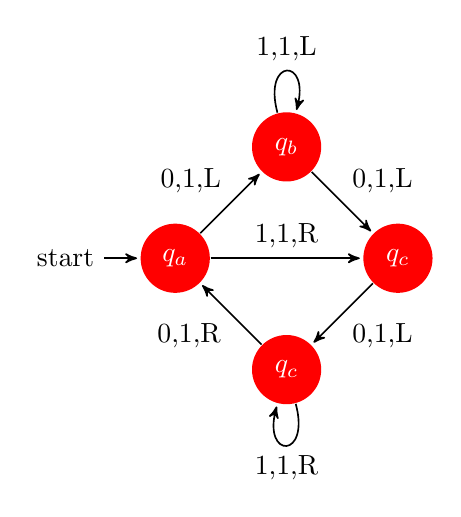
\begin{tikzpicture}[->,>=stealth',shorten >=1pt,auto,node distance=2cm,
                    semithick]
  \tikzstyle{every state}=[fill=red,draw=none,text=white]

  \node[initial,state] (A)                    {$q_a$};
  \node[state]         (B) [above right of=A] {$q_b$};
  \node[state]         (D) [below right of=A] {$q_c$};
  \node[state]         (C) [below right of=B] {$q_c$};
%  \node[state]         (E) [left of=A]       {$q_d$};

  \path (A) edge              node {0,1,L} (B)
            edge              node {1,1,R} (C)
        (B) edge [loop above] node {1,1,L} (B)
            edge              node {0,1,L} (C)
        (C) edge              node {0,1,L} (D)
%            edge [bend left]  node {1,0,R} (E)
        (D) edge [loop below] node {1,1,R} (D)
            edge              node {0,1,R} (A);
%        (E) edge [bend left]  node {1,0,R} (A);
\end{tikzpicture}
\caption{Moore's Machine example}
\label{moore}
\end{center}
\end{figure}
% problema del commesso viaggiatore
% Is it a partial observable problem?
% NTH: RNN

\paragraph{Datasets and Inputs}

% The dataset(s) and/or input(s) to be used in the project are thoroughly described. Information such as how the dataset or input is (was) obtained, and the characteristics of the dataset or input, should be included. It should be clear how the dataset(s) or input(s) will be used in the project and whether their use is appropriate given the context of the problem.

% how the rtl model is generated
% big number of states

Functional verification is normally done using Electronic Design Automation (EDA) software for performing verification and for measuring DUT's coverage. For this project we can't use this approach because these softwares are under license and because a single test requires a significant amount of time, due to the modelization of the hardware DUT. For overcoming this problem we will generate a generic and parametrizable model of a DUT: we will design a python function taking as input the number of states, the number of inputs, and will return the corresponding Moore's Machine (quite similar to an oriented graph). This approach will give us also the opportunity to progressively increase the number of states of the DUT, and then understand how our solution is able to solve the problem.

\paragraph{Solution Statement}

% Student clearly describes a solution to the problem. The solution is applicable to the project domain and appropriate for the dataset(s) or input(s) given. Additionally, the solution is quantifiable, measurable, and replicable.

% RL with actor-critic
% RL model using the terms in https://en.wikipedia.org/wiki/Moore_machine
In the schematic in figure \ref{RI} we can see how I'm approaching the problem: my goal will be to design an Agent capable of forcing some input (actions) on the DUT (Environment), based on the register values (state). The reward will be a function of the coverage, which is an indicator of states explored.
As previously said, the problem will be solved using reinforcement learning: the episode will be a test, and a step of the episode corresponds to a test's cycle (in the schematic is not shown, but registers have clock input). In particular the actor-critic method as in the \href{https://arxiv.org/pdf/1509.02971.pdf}{DDPG paper} will be employed. I'm very willing to master this method because it's very new and seems to be perfect for solving this problem, as it may have a really big number of states. My goal is to try different configurations of DUT, varying the input size between 2 and 100, and the states number between 10 and 1000.
\begin{figure}
\begin{center}
\tikzset{every picture/.style={line width=0.75pt}} %set default line width to 0.75pt        
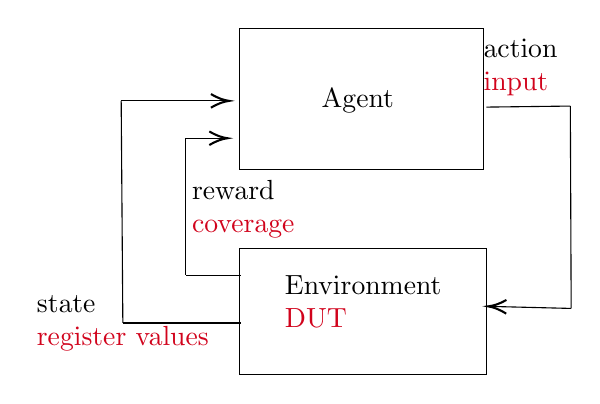
\begin{tikzpicture}[x=0.75pt,y=0.75pt,yscale=-1,xscale=0.8]
%uncomment if require: \path (0,300); %set diagram left start at 0, and has height of 300

%Straight Lines [id:da9594583335701603] 
\draw    (164.5,130) -- (227.5,130) ;
\draw [shift={(229.5,130)}, rotate = 180] [color={rgb, 255:red, 0; green, 0; blue, 0 }  ][line width=0.75]    (10.93,-3.29) .. controls (6.95,-1.4) and (3.31,-0.3) .. (0,0) .. controls (3.31,0.3) and (6.95,1.4) .. (10.93,3.29)   ;

%Shape: Rectangle [id:dp94563734044778] 
\draw   (236,95) -- (382.5,95) -- (382.5,163) -- (236,163) -- cycle ;
%Shape: Rectangle [id:dp11834384088600869] 
\draw   (236,201) -- (384.5,201) -- (384.5,262) -- (236,262) -- cycle ;
%Straight Lines [id:da3011906563331679] 
\draw    (435,132.5) -- (435.5,230) ;


%Straight Lines [id:da2080054398331841] 
\draw    (435.5,230) -- (387.5,229.04) ;
\draw [shift={(385.5,229)}, rotate = 361.15] [color={rgb, 255:red, 0; green, 0; blue, 0 }  ][line width=0.75]    (10.93,-3.29) .. controls (6.95,-1.4) and (3.31,-0.3) .. (0,0) .. controls (3.31,0.3) and (6.95,1.4) .. (10.93,3.29)   ;

%Straight Lines [id:da2418080495725663] 
\draw    (203.5,214) -- (236.5,214) ;


%Straight Lines [id:da2403153951084427] 
\draw    (203.5,148) -- (203.5,214) ;


%Straight Lines [id:da26911747717628987] 
\draw    (203.5,148) -- (226.5,148) ;
\draw [shift={(228.5,148)}, rotate = 180] [color={rgb, 255:red, 0; green, 0; blue, 0 }  ][line width=0.75]    (10.93,-3.29) .. controls (6.95,-1.4) and (3.31,-0.3) .. (0,0) .. controls (3.31,0.3) and (6.95,1.4) .. (10.93,3.29)   ;

%Straight Lines [id:da8156632977564808] 
\draw    (384.5,133) -- (435,132.5) ;


%Straight Lines [id:da9972423669598849] 
\draw    (164.5,130) -- (165.5,237) ;


%Straight Lines [id:da15454461757044902] 
\draw    (165.5,237) -- (236.5,237) ;



% Text Node
\draw (165.5,237) node  [align=left] {state\\\textcolor[rgb]{0.82,0.01,0.11}{register values}};
% Text Node
\draw (307,130) node  [align=left] {Agent};
% Text Node
\draw (405,114) node  [align=left] {action\\\textcolor[rgb]{0.82,0.01,0.11}{input}};
% Text Node
\draw (310.25,226.5) node  [align=left] {Environment\\\textcolor[rgb]{0.82,0.01,0.11}{DUT}};
% Text Node
\draw (238,182) node  [align=left] {reward\\\textcolor[rgb]{0.82,0.01,0.11}{coverage}};


\end{tikzpicture}
\caption{DUT as part of Reinforcement Learning}
\label{RI}
\end{center}
\end{figure}

\paragraph{Benchmark Model}
% A benchmark model is provided that relates to the domain, problem statement, and intended solution. Ideally, the student's benchmark model provides context for existing methods or known information in the domain and problem given, which can then be objectively compared to the student's solution. The benchmark model is clearly defined and measurable.

% TODO search some papers results to compare
When performing functional verification we ideally want to reach 100\% coverage: this will be our ideal target, which normally is obtained merging the coverage of thousands of random tests.
The state of the art of machine learning applied to functional coverage is represented from the work done at \href{http://www.research.ibm.com/haifa/dept/vst/hvt_psvtva.shtml}{IBM}. Another scientific reference used for background knowledge is \href{https://www.researchgate.net/publication/220306081_Coverage-Directed_Test_Generation_Automated_by_Machine_Learning_-_A_Review}{this paper}: an important outcome are the coverage results. From these tables we can deduct that 80\% of coverage maybe considered as really good. % Both references have been used for insipring and ....


\paragraph{Evaluation Metrics}
% Student proposes at least one evaluation metric that can be used to quantify the performance of both the benchmark model and the solution model presented. The evaluation metric(s) proposed are appropriate given the context of the data, the problem statement, and the intended solution.

% states vs NN complexity
% cycles for reaching 90% coverage compared to random stimuli

We have different metrics for evaluating the agent. The more important one is the coverage, which returns us the percentage of stimulated states of the DUT. Another one is the number of cycles needed to reach the 80\% coverage; these results have particular relevance when compared with respect to the results obtained using a completely random generator. Finally we can underline how the complexity of agent (actor-critic neural networks weights) scale with the increasing of DUT's complexity.

\paragraph{Project Design}
% Student summarizes a theoretical workflow for approaching a solution given the problem. Discussion is made as to what strategies may be employed, what analysis of the data might be required, or which algorithms will be considered. The workflow and discussion provided align with the qualities of the project. Small visualizations, pseudocode, or diagrams are encouraged but not required.

The starting point will be the code obtained form the project ``Tech a Quadcopter How to Fly'', and then reuse the actor-critic approach. The first step of the project is to generate the parametrizable DUT model, which will be used as the environment of the problem. Then a series of events will be generated and the goal will be to generate a test (or a series of tests) capable of learning how to cover the DUT. The project will be hosted on github in \href{git@github.com:birio/capstone_project.git}{this} repository.

% \subsubsection*{Presentation}
% How I will structure the final report
% list of docs and kind of docs I will submit
% how I generated the pdf from latex

% Proposal follows a well-organized structure and would be readily understood by its intended audience. Each section is written in a clear, concise and specific manner. Few grammatical and spelling mistakes are present. All resources used and referenced are properly cited. 
 
\end{document}
